With the state-space model of the HDT defined, the next step is to design a control strategy that ensures the desired performance. 

\begin{figure}[t!]
    \centering
    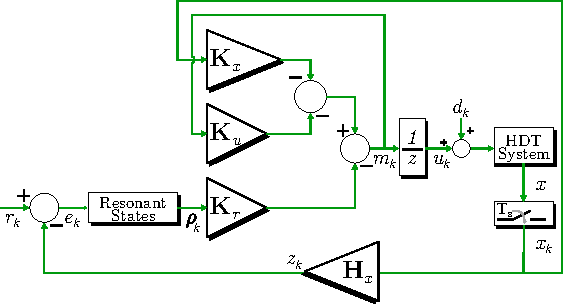
\includegraphics[width=\columnwidth]{Images/Control_Diagram.pdf} 
    \caption{Block diagram of the proposed control strategy for the HDT.}
    \label{fig:Control_Diagram}
\end{figure}

\begin{figure*}[t!]
    \centering
    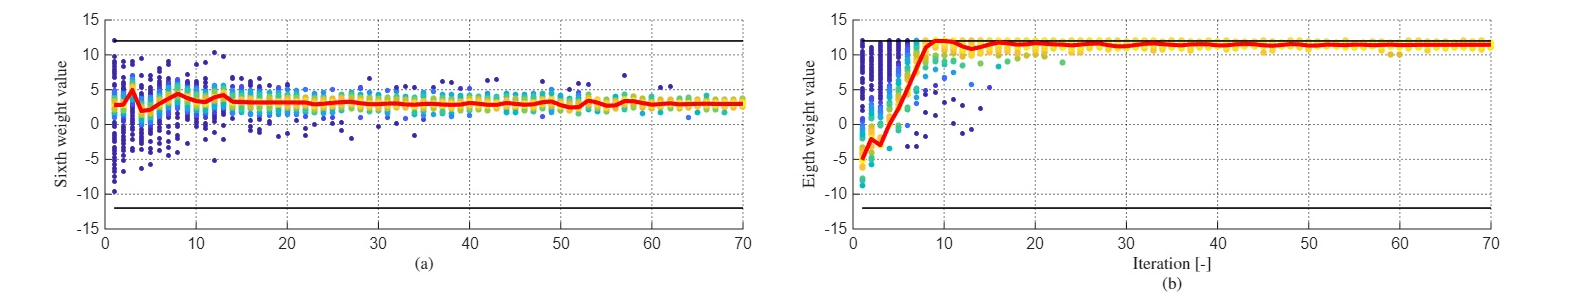
\includegraphics[width = \textwidth]{Images/w6_w8_iterations.pdf}
    \caption{Convergence of exponents over the PSO iterations. (a) Exponent $q_6$ associated with the parallel converter inductor current $v_{cp,\alpha\beta}$. (b) Exponent $q_8$ associated with the first resonant state of the error $e1v_{cs,\alpha\beta}$.}
    \label{fig:PSO_Convergence}
\end{figure*}

\subsection{Proposed Control Strategy}

The proposed control strategy is based on a state feedback controller which is designed using the augmented state-space model of the HDT, defined in the \Cref{eq:Aug_Model}. The control strategy aims to achieve zero steady-state error for sinusoidal references. The state feedback controller is designed using the discrete LQR approach given by:
\begin{equation}
    \mathbf{K} = \text{dlqr}(\mathbf{A}_{d,delay}, \mathbf{B}_{d,\text{aug}}, \mathbf{Q}, \mathbf{R})
\end{equation}
where $\mathbf{Q}\in\mathbb{R}^{11}$ and $\mathbf{R}\in\mathbb{R}^4 = \mathbf{I}$ are the state and input weighting matrices, respectively. The gain matrix is partitioned into three sub-matrices: $\mathbf{K}_x$, $\mathbf{K}_u$ and $\mathbf{K}_r$ for convenience. The block diagram of the proposed control strategy is shown in \Cref{fig:Control_Diagram}. With the partitioned gain matrices defined, the control input can be expressed as:
\begin{equation}
    u_k = -\mathbf{K}_x
    \begin{bmatrix}
        x_k\\
        m_k
    \end{bmatrix} + \mathbf{K}_u m_k - \mathbf{K}_r \rho_k
\end{equation}
where $\mathbf{K}_x$ is the state feedback gain matrix, $\mathbf{K}_u$ is the previous control input gain matrix and $\mathbf{K}_r$ is the resonant states gain matrix.

As mentioned before, the proposed control strategy includes resonant states to ensure zero steady-state error for sinusoidal references. The resonant states are defined by the following differential equation:
\begin{equation}
    \dfrac{d\,\rho(t)}{dt} = 
    \underbrace{
    \begin{bmatrix}
        0 & \omega \\
        -\omega & 0
    \end{bmatrix}
    }_{\mathbf{A}_r}
    \rho(t) + 
    \underbrace{
    \begin{bmatrix}
        1\\
        0
    \end{bmatrix}
    }_{\mathbf{B}_r}
    e(t)
\end{equation}
where $\omega$ is the nominal angular frequency and $e(t)$ is the error vector between the reference and the measured output. Each of the references signals has two resonant states associated with it, meaning that for the HDT control, there are eight resonant states in total (4 for the $ev_{cs,\alpha\beta}$ and 4 for the $i_{fp,\alpha\beta}$). This can be expressed as:
\begin{align}
    \dfrac{d\,\rho(t)}{dt} &= \text{diag}(\mathbf{A}_r, \mathbf{A}_r, \mathbf{A}_r, \mathbf{A}_r)\rho(t)\\
    &+ \text{diag}(\mathbf{B}_r, \mathbf{B}_r, \mathbf{B}_r, \mathbf{B}_r)e(t)
\end{align}

These resonant states are then discretized using a ZOH giving the matrices $\mathbf{A}_{rd}$ and $\mathbf{B}_{rd}$. The augmented state-space model of the resonant states can be expressed as:
\begin{align}
    \begin{aligned}
        \begin{bmatrix}
            x_{k + 1}\\
            m_{k + 1}\\
            \rho_{k + 1}
        \end{bmatrix}
        &=
        \begin{bmatrix}
            \mathbf{A}_{d,delay} & \mathbf{0} \\
            \mathbf{B}_{rd}\mathbf{H}_x & \mathbf{A}_{rd}
        \end{bmatrix}
        \begin{bmatrix}
            x_k\\
            m_k\\
            \rho_k
        \end{bmatrix}
        +
        \begin{bmatrix}
            \mathbf{B}_{d,\text{aug}}\\
            \mathbf{0}
        \end{bmatrix}
        \begin{bmatrix}
            u_k\\
            e_k
        \end{bmatrix}
        \\
        y_k &= 
        \begin{bmatrix}
            \mathbf{C} & \mathbf{0}
        \end{bmatrix}
        \begin{bmatrix}
            x_K\\
            m_k\\
            \rho_k
        \end{bmatrix}
    \end{aligned}
\end{align}
where $\mathbf{H}_x$ selects the states from the HDT state vector that are imposed to follow references.

\subsection{Particle Swarm Optimization}

To facilitate the tuning of the state feedback gain matrix $\mathbf{K}$ by adjusting $\mathbf{Q}$, the PSO algorithm is employed to optimize the weights associated with each state in the cost function. The PSO algorithm is a population-based optimization technique inspired by the social behavior of birds and fish. It consists of a swarm of particles, where each particle represents a potential solution to the optimization problem, in this case, the vector of exponents $q_l$, where $l\in\left[1,2,...,11\right]$. The particles move through the search space, updating their positions based on their own experience and the experience of their neighbors. The velocity and position of each particle are updated using the following equations:
\begin{align}
    \begin{aligned}
        v_j(i + 1) &= K_{ap}\left(v_j(i) + c_1 r_1 (pbest_j - x_j(i)) \right.\\
        & \left. + c_2 r_2 (gbest - x_j(i))\right)\\
        x_j(i + 1) &= x_j(i) + v_j(i + 1)
    \end{aligned}
\end{align}
where $v_j(i)$ is the velocity of particle $j$ at iteration $i$, $x_j(i)$ is the position of particle $j$ at iteration $i$, $pbest_j$ is the best position found by particle $j$, $gbest$ is the best position found by the entire swarm, $c_1$ and $c_2$ are cognitive and social acceleration coefficients, $r_1$ and $r_2$ are random numbers uniformly distributed in the range [0, 1], and $K_{ap}$ is the constriction factor given by:
\begin{equation}
    K_{ap} = \dfrac{2}{\left|2 - \phi - \sqrt{\phi^2 - 4\phi}\right|}
\end{equation}
where $\phi = c_1 + c_2 > 4$ is a constant that ensures convergence.

The PSO algorithm iteratively updates the positions and velocities of the particles until a stopping criterion is met, sin this case, the maximum of iteration number. The best position found by the swarm is considered the optimal solution to the optimization problem.

\begin{figure}[t!]
    \centering
    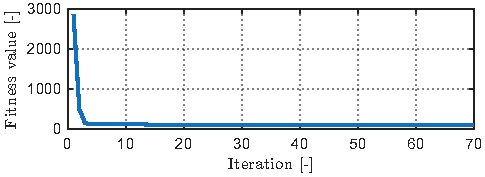
\includegraphics[]{Images/Fitness_iterations.pdf}
    \caption{Convergence of the fitness value over the PSO iterations.}
    \label{fig:PSO_Fitness}
\end{figure}

\subsection{PSO Performance Index}

The performance index used for the PSO optimization is a cost function that considers both the transient and steady-state performance of the HDT. The cost function is defined as:
\begin{equation}
    J = \dfrac{1}{N} \sum_{i=1}^{N} |e_k|^2 + \beta \Delta u_k^2
\end{equation}
where $N$ is the number of samples in the simulation, $e_k$ is the error vector at sample $k$, $\Delta u_k$ is the change in control input at sample $k$, and $\beta$ is a weighting factor that balances the importance of the transient and steady-state performance.

The weights are defined as:
\begin{equation}
    w_i = 10^{q_i}
\end{equation}
where $w_i$ is the weight associated with state $i$, and $q_i$ is the exponent to be optimized. The weights are used to scale the states in the cost function, allowing the PSO algorithm to prioritize certain states over others. The optimization variables lie within the range $[-20,20]$ including the absorbing walls boundaries. The PSO parameters used for the optimization are listed in Table \ref{tab:PSO_Parameters}.

\begin{table}[h!]
    \centering
    \caption{PSO parameters used for the optimization of the control gains.}
    \label{tab:PSO_Parameters}
    \begin{tabular}{|l|c|}
        \hline
        \textbf{Parameter} & \textbf{Value}\\
        \hline\hline
        Number of particles & 100\\
        Maximum number of iterations & 70\\
        Absorbing walls boundaries & $[-12, 12]$\\
        Cognitive acceleration coefficient ($c_1$) & 2.05\\
        Social acceleration coefficient ($c_2$) & 2.05\\
        Maximum weight exponent for states ($q_{max}$) & 4.5\\
        Damping ratio for resonant states ($\xi$) & 0.01\\
        \hline
    \end{tabular}
\end{table}

After running the PSO algorithm, each of the state weights exponents ($q_i$) are given by:
\begin{align}
    \begin{aligned}
        q_1 &= -0.7009 & q_2 &= -3.2101 & q_3 &= -2.9568\\
        q_4 &= 3.4510 & q_5 &= -3.3684 & q_6 &= 2.9170\\
        q_7 &= -5.9347 & q_8 &= 11.4511 & q_9&= 11.4543\\
        q_{10} &= 5.7987 & q_{11} &= 0.5847
    \end{aligned}
\end{align}

\begin{figure*}
    \centering
    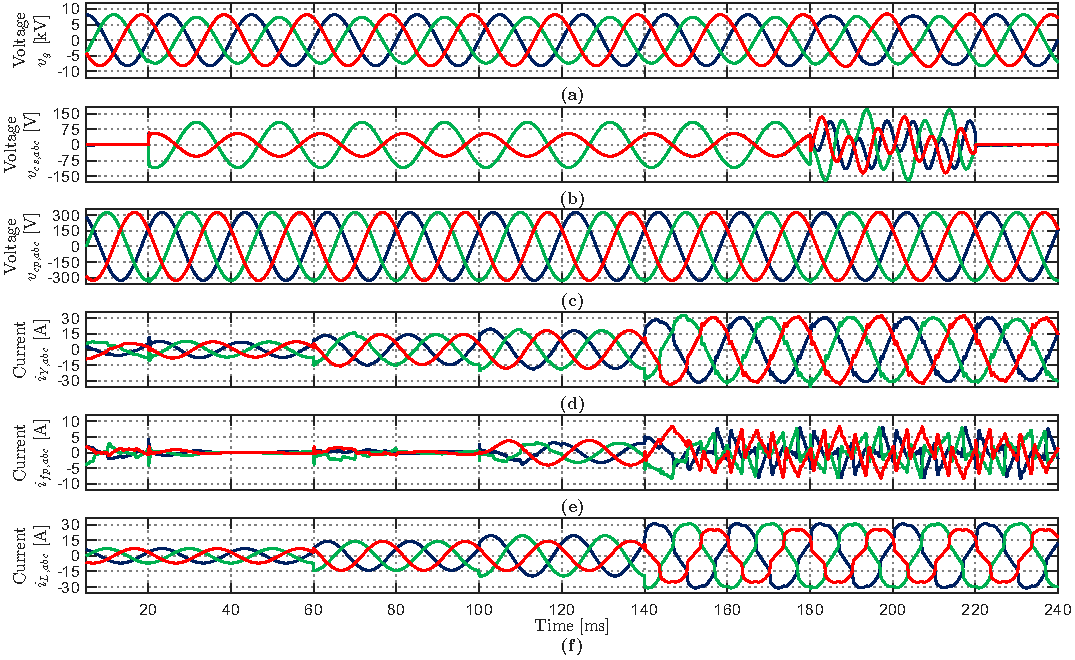
\includegraphics[width=\textwidth]{Images/Simulation_Results.pdf}
    \caption{Simulation results for the proposed control strategy under grid and load disturbances. (a) Grid voltage $v_g^{abc}$, (b) Series converter capacitor voltage $v_{cs}^{abc}$, (c) Parallel converter capacitor voltage $v_{cp}^{abc}$, (d) Series converter inductor current $i_{cs}^{abc}$, (e) Secondary side transformer current $i_Y^{abc}$, (f) Parallel converter inductor current $i_{cp}^{abc}$}
    \label{fig:Sim_results}
\end{figure*}